\begin{tikzpicture}[x=1cm,y=1cm,font=\small\sffamily]
\path[use as bounding box] (0,-.4) rectangle (14,5.9);
\node[anchor=west,font=\bfseries] at (.2,5.6){A / Distinct partners};
\foreach \x in {.5,1.2,1.9}\shade[ball color=Blue!50] (\x,4.6) circle (.17);
\foreach \x in {3.5,4.2,4.9}\shade[ball color=Green!50] (\x,4.6) circle (.17);
\draw[Blue!35] (1.2,4.4)--(3.5,4.4);
\draw[Blue!35,dashed] (1.2,4.4)--(4.2,4.4);
\node[align=center] at (2.7,3.5){ordered species roles: $AB$ eligible pairs\\$\alpha_{AB}=(k/\Omega)AB$};
\node[anchor=west,font=\bfseries] at (7.1,5.6){B / Two identical partners};
\foreach \x in {7.6,8.4,9.2}\shade[ball color=Blue!50] (\x,4.6) circle (.17);
\draw[Blue!35] (7.6,4.3)--(8.4,4.3);
\draw[Blue!35,dashed] (8.4,4.15)--(9.2,4.15);
\node[align=center] at (10.3,3.5){unordered pairs: $\binom A2$\\$\alpha_{AA}=(2k/\Omega)\binom A2$};
\draw[Blue!25] (.2,2.6)--(13.8,2.6);
\node[align=left,anchor=north west,text width=6.4cm] at (.3,2.2){\textbf{Declared molar event law}\\
distinct: $v=kab$\\identical: $v=ka^2$\\$\Omega=N_{\rm A}V$; $k$: L/(mol$\cdot$time)};
\node[align=left,anchor=north west,text width=6.2cm] at (7.2,2.2){\textbf{Consumption is separate}\\
$2A\to P$ consumes two copies per event.\\
$\dot a=-2v$, not $-v$.\\
Count one has no eligible identical pair.};
\end{tikzpicture}
